% \documentclass[aspectratio=169,notes]{beamer}
\documentclass[aspectratio=169]{beamer}
\usetheme[faculty=phil]{fibeamer}
\usepackage{polyglossia}
\setmainlanguage{english} %% main locale instead of `english`, you
%% can typeset the presentation in either Czech or Slovak,
%% respectively.
\setotherlanguages{russian} %% The additional keys allow
%%
%%   \begin{otherlanguage}{czech}   ... \end{otherlanguage}
%%   \begin{otherlanguage}{slovak}  ... \end{otherlanguage}
%%
%% These macros specify information about the presentation
\title[Theoretical Mechanics]{Theoretical Mechanics, Lab 8: DYN PART [NON]INERT} %% that will be typeset on the
\subtitle{Intro to Dynamics
\\ Particle Dynamics for inertial systems \\ Particle Dynamics for non-inertial systems 
         } %% title page.
\author{Oleg Bulichev}
%% These additional packages are used within the document:
\usepackage{ragged2e}  % `\justifying` text
\usepackage{booktabs}  % Tables
\usepackage{tabularx}
\usepackage{tikz}      % Diagrams
\usetikzlibrary{calc, shapes, backgrounds}
\usepackage{amsmath, amssymb}
\usepackage{url}       % `\url`s
\usepackage{listings}  % Code listings
% \usepackage{subfigure}
\usepackage{floatrow}
\usepackage{subcaption}
\usepackage{mathtools}
\usepackage{todonotes}
\usepackage{fontspec}
\usepackage{multicol}
\usepackage{pdfpages}
\usepackage{wrapfig}
\usepackage{animate}
\usepackage{booktabs}
\usepackage{multirow}
% \usepackage{graphicx}
\usepackage{colortbl}
\usepackage{catchfilebetweentags}
\usepackage{makecell}
\graphicspath{{resources/}}
\frenchspacing

\setbeamertemplate{caption}[numbered]
\usetikzlibrary{graphs}

% \usepackage[backend=biber,style=ieee,autocite=footnote]{biblatex}
% \addbibresource{biblio.bib}
% \DefineBibliographyStrings{english}{%
%   bibliography = {References},}

\newcommand{\oleg}[2][] {\todo[color=red, #1] {OLEG:\\ #2}}
\newcommand{\fbckg}[1]{\usebackgroundtemplate{\includegraphics[width=\paperwidth]{#1}}}%frame background

\usepackage[framemethod=TikZ]{mdframed}
\newcommand{\dbox}[1]{
\begin{mdframed}[roundcorner=3pt, backgroundcolor=yellow, linewidth=0]
\vspace{1mm}
{#1}
\vspace{1mm}
\end{mdframed}
}

\begin{document}
\setlength{\abovedisplayskip}{0pt}
\setlength{\belowdisplayskip}{0pt}
\setlength{\abovedisplayshortskip}{0pt}
\setlength{\belowdisplayshortskip}{0pt}

\fbckg{fibeamer/figs/title_page.png}
\frame[c]{\setcounter{framenumber}{0}
    \usebeamerfont{title}%
    \usebeamercolor[fg]{title}%
    \begin{minipage}[b][6.5\baselineskip][b]{\textwidth}%
        \textcolor{black}{\raggedright\inserttitle}
    \end{minipage}
    % \vskip-1.5\baselineskip

    \usebeamerfont{subtitle}%
    \usebeamercolor[fg]{framesubtitle}%
    \begin{minipage}[b][3\baselineskip][b]{\textwidth}
        \raggedright%
        \insertsubtitle%
    \end{minipage}
    \vskip.25\baselineskip
}
%   \frame[c]{\maketitle}

\fbckg{fibeamer/figs/common.png}


\section*{Theory}

\begin{frame}[t]{Forward Dynamics  (2nd dynamics problem)}
\framesubtitle{}
    We know applied forces and want to find equation of motion.
    \begin{figure}[H]
        \centering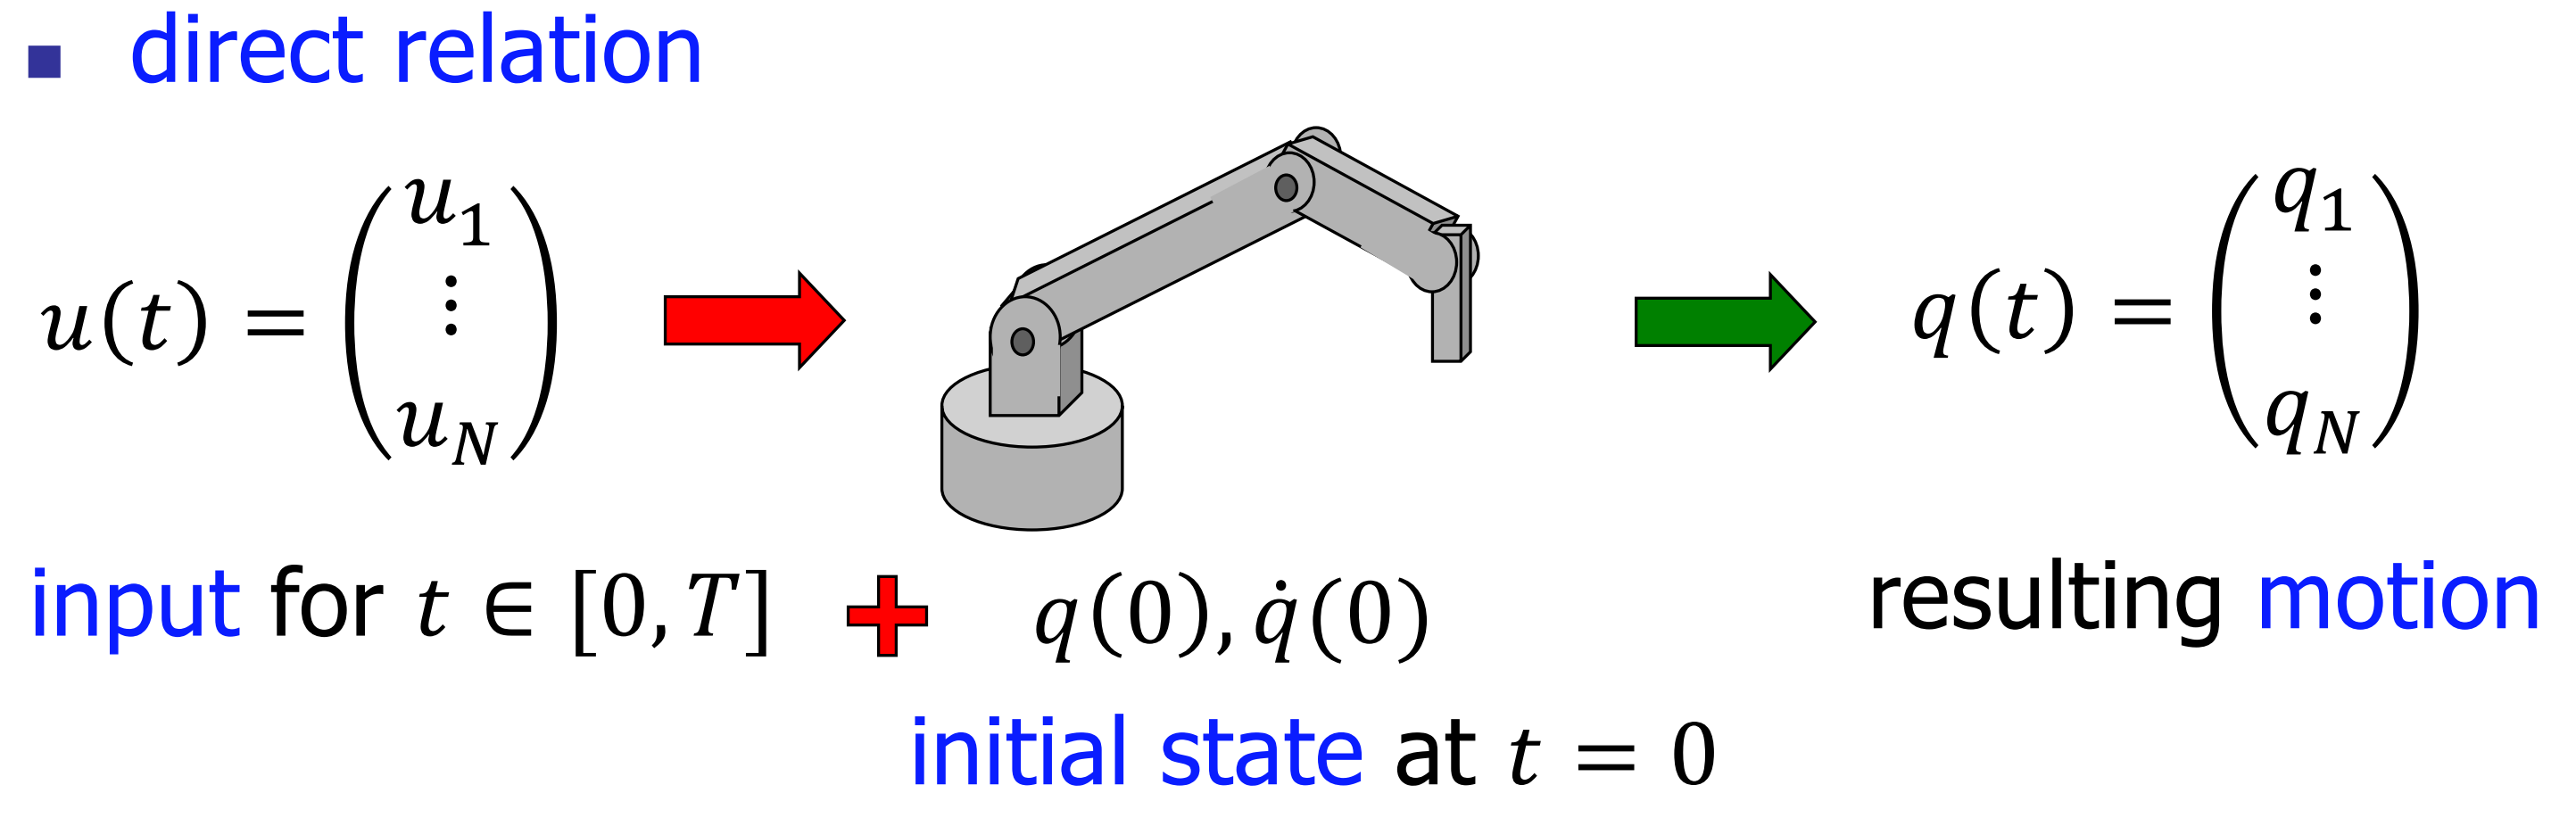
\includegraphics[height=4cm,width=1\textwidth,keepaspectratio]{forward_dynamics.png}
        % \caption{caption_name}
        \label{fig:forward_dynamics.png}
    \end{figure}
\end{frame}

\begin{frame}[t]{Inverse Dynamics  (1st dynamics problem)}
    \framesubtitle{}
        We know equation of motion ($X,\ \dot{X},\ \ddot{X}$) and we want to find applied forces respect to time.
        \begin{figure}[H]
            \centering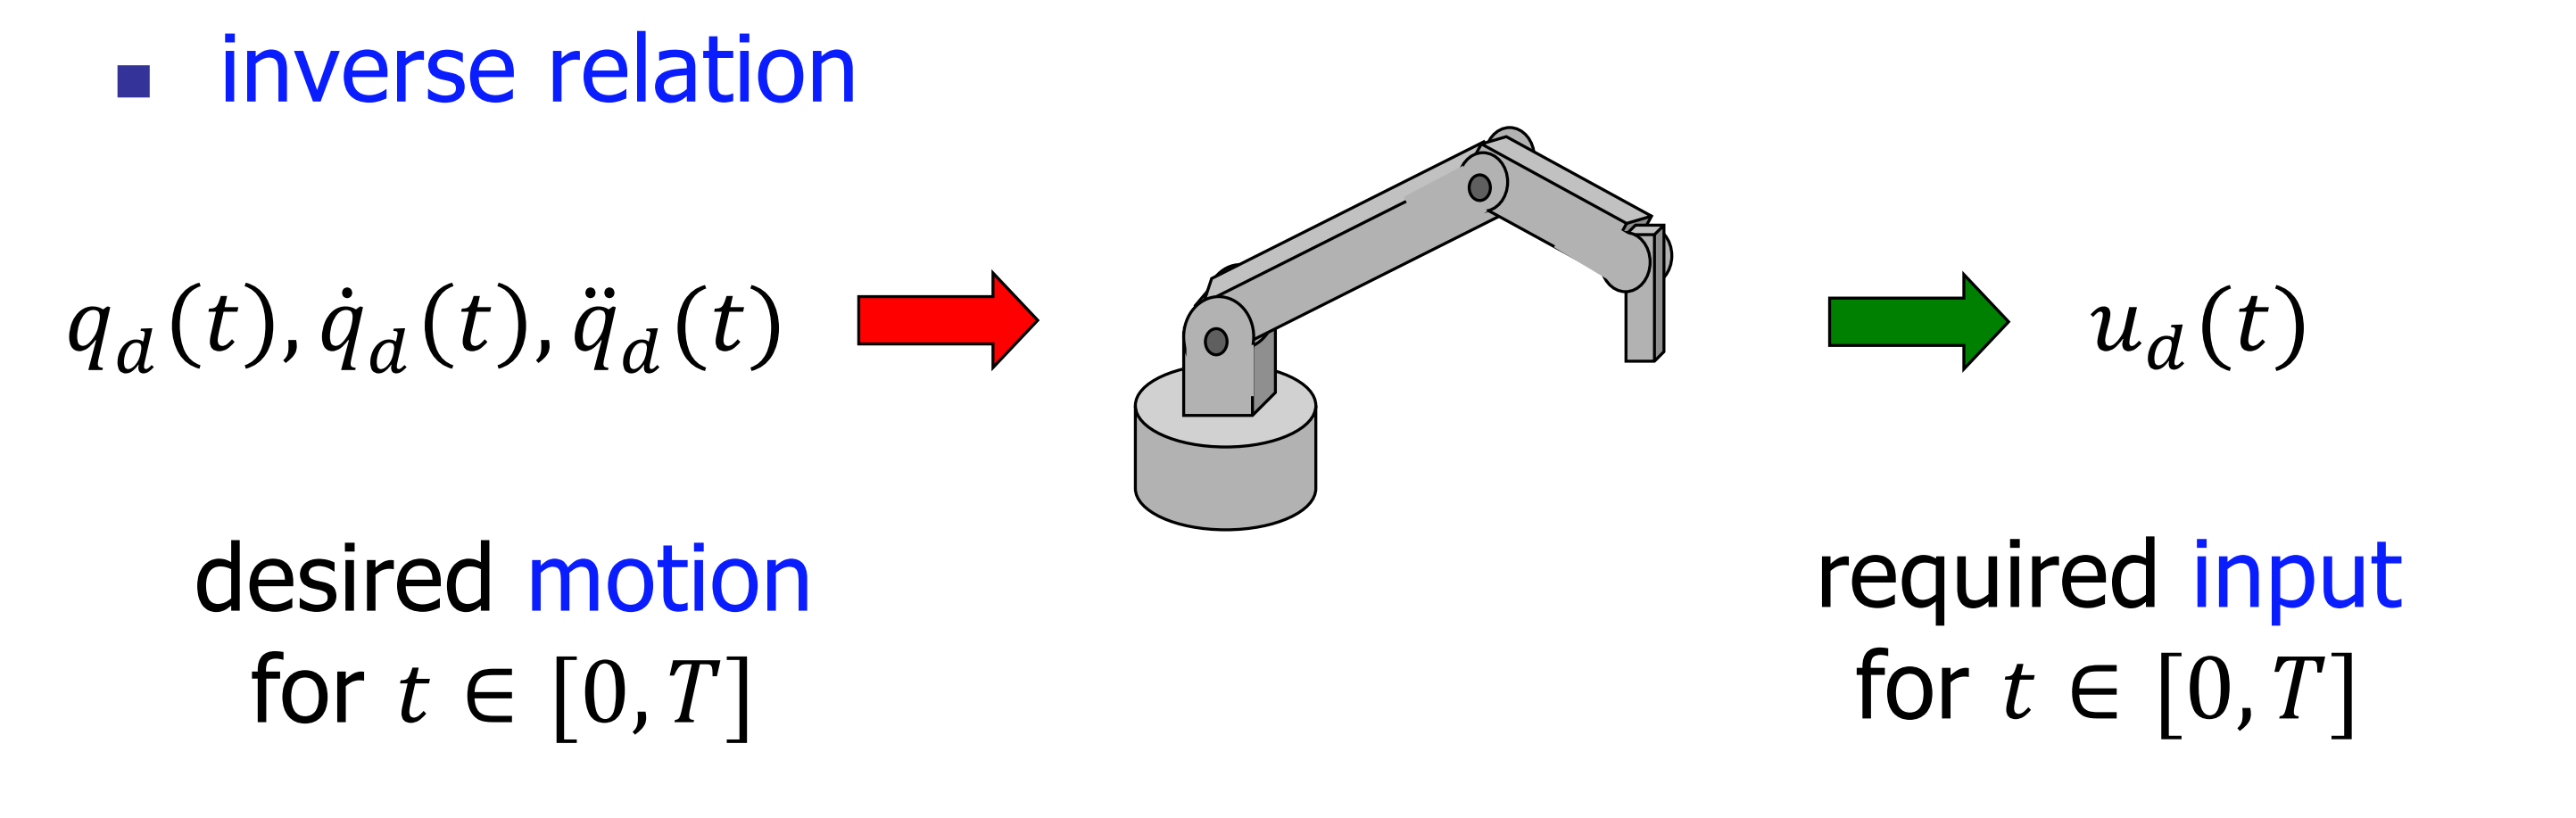
\includegraphics[height=4cm,width=1\textwidth,keepaspectratio]{inverse_dynamics.png}
            % \caption{caption_name}
            \label{fig:inverse_dynamics.png}
        \end{figure}
    \end{frame}

\begin{frame}[t]{Method of solving forward dynamics}
    \framesubtitle{}
    \vspace*{-0.6cm}
    \begin{multicols}{2}
        \begin{enumerate}
            \item Analyze the system
                  \begin{itemize}
                      \small
                      \item Show the frame of reference
                      \item Show the particle in an common position
                      \item Show the initial, final position of the particle
                      \item Write the initial, final conditions
                  \end{itemize}
            \item Analyze forces
                  \begin{itemize}
                      \small
                      \item Make a list of all the forces
                      \item Specify the formula for calculating the forces
                      \item Show all forces on the scheme
                  \end{itemize}
            \item Solve the problem
                  \begin{itemize}
                      \small
                      \item Write the differential equations of motion
                      \item Find a common solution
                      \item Substitute the initial conditions to find the
                            constants of integration
                      \item Substitute other conditions to find the answer
                  \end{itemize}
        \end{enumerate}
    \end{multicols}
\end{frame}

\begin{frame}[t]{Force types}
    \framesubtitle{}
    In our course we will use only:
    \begin{itemize}
        \setbeamertemplate{itemize item}{$\Rightarrow$}
        \item Constant force $\vec{F}=const$
        \item Time dependent force $\vec{F}=\vec{F}(t)$
        \item Velocity dependent force $\vec{F}=\vec{F}(\dot{\vec{r}})$
        \item Position dependent force $\vec{F}=\vec{F}(t,\vec{r},\dot{\vec{r}}) \Rightarrow \left\{\begin{matrix*}[l]
                      F_x = F_x(t,x,y,\dot{x},\dot{y})\\
                      F_y = F_y(t,x,y,\dot{x},\dot{y})
                  \end{matrix*}\right.$
    \end{itemize}
\end{frame}

\begin{frame}[t]{Force types}
    \framesubtitle{Constant force}
    \vspace*{-0.6cm}
    \begin{center}
        \begin{figure}[H]
            \centering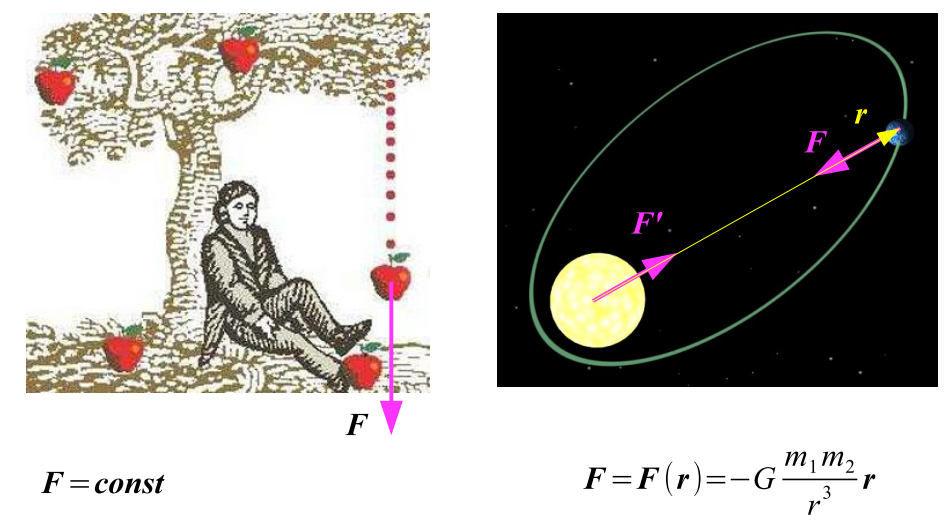
\includegraphics[height=6cm,width=1\textwidth,keepaspectratio]{image12.png}
            \label{fig:image12}
        \end{figure}
    \end{center}
\end{frame}

\begin{frame}[t]{Force types}
    \framesubtitle{Resistance force}
    \vspace*{-0.6cm}
    \begin{center}
        \begin{figure}[H]
            \centering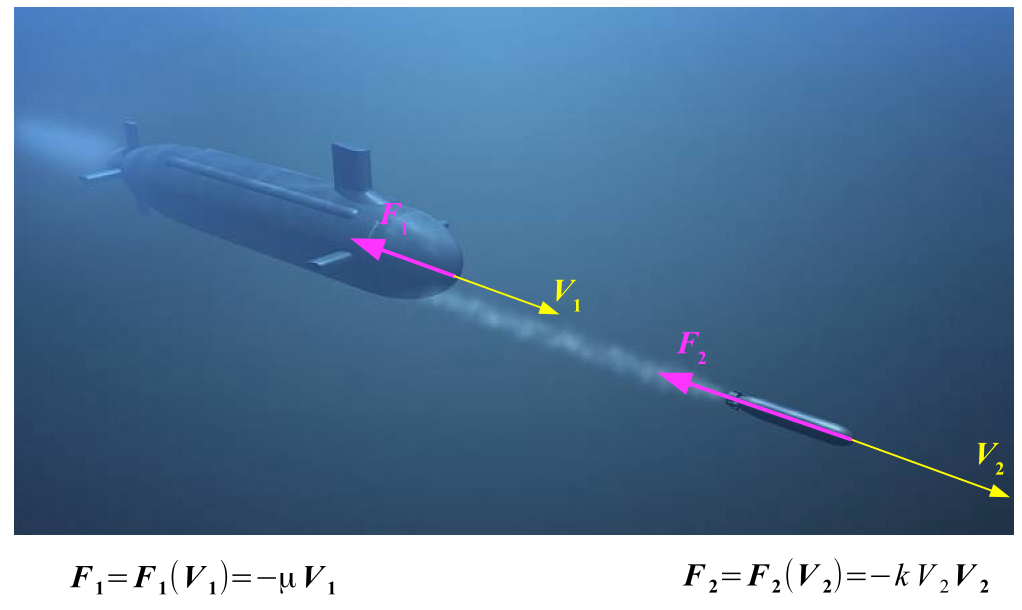
\includegraphics[height=6cm,width=1\textwidth,keepaspectratio]{image23.png}
            \label{fig:image23}
        \end{figure}
    \end{center}
\end{frame}

\begin{frame}[t]{Force types}
    \framesubtitle{Controlled force}
    \vspace*{-0.6cm}
    \begin{center}
        \begin{figure}[H]
            \centering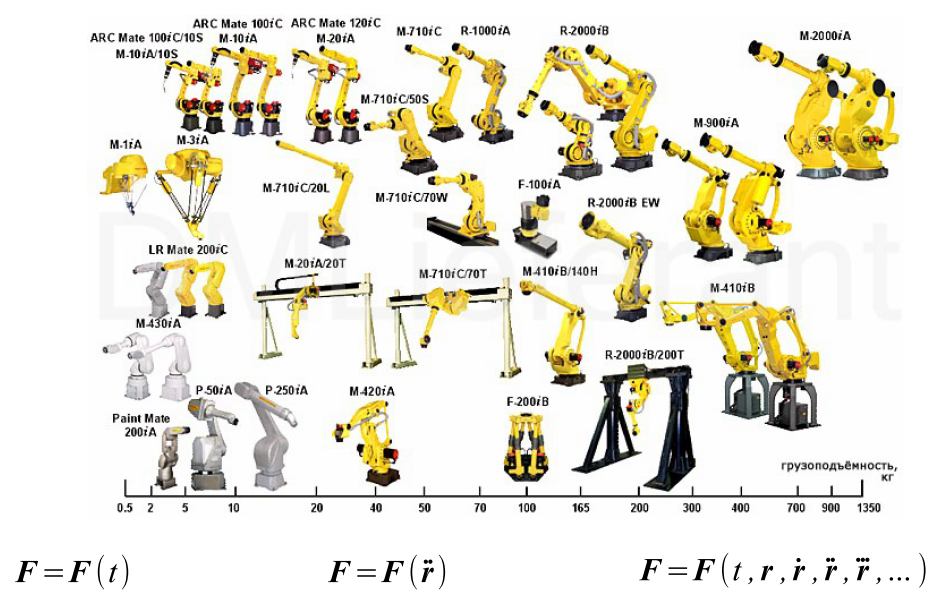
\includegraphics[height=6cm,width=1\textwidth,keepaspectratio]{image22.png}
            \label{fig:image22}
        \end{figure}
    \end{center}
\end{frame}

\begin{frame}[t]{Typical differential equations}
    \framesubtitle{Constant and time dependent forces}
    \vspace*{-0.6cm}
    \begin{center}
        \begin{figure}[H]
            \centering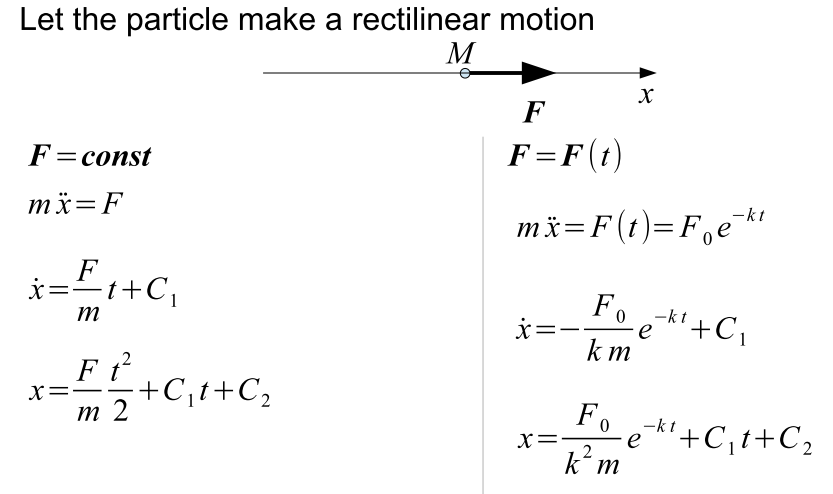
\includegraphics[height=5cm,width=1\textwidth,keepaspectratio]{image18.png}
            \label{fig:image18}
        \end{figure}
    \end{center}
\end{frame}

\begin{frame}[t]{Typical differential equations}
    \framesubtitle{Resistance force: 1D case}
    \vspace*{-0.6cm}
    \begin{center}
        \begin{figure}[H]
            \centering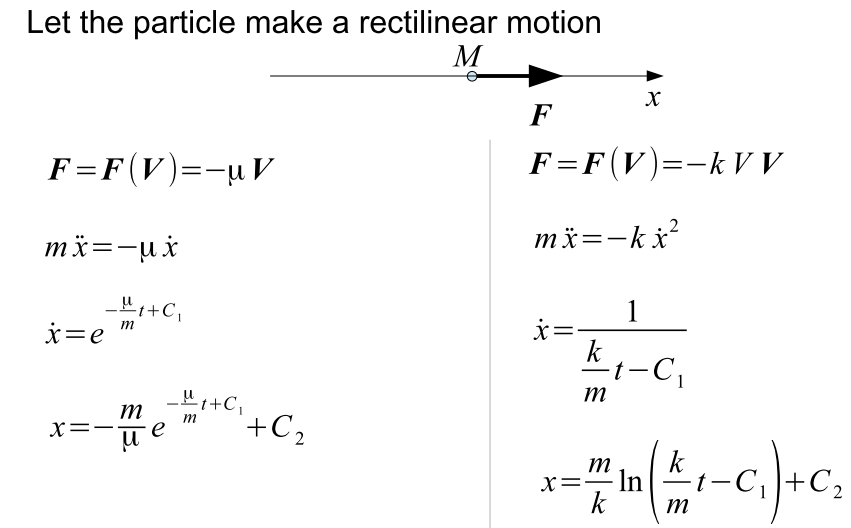
\includegraphics[height=5cm,width=1\textwidth,keepaspectratio]{image11.png}
            \label{fig:image11}
        \end{figure}
    \end{center}
\end{frame}

\begin{frame}[t]{Typical differential equations}
    \framesubtitle{Resistance force: 2D case}
    \vspace*{-0.6cm}
    \begin{center}
        \begin{figure}[H]
            \centering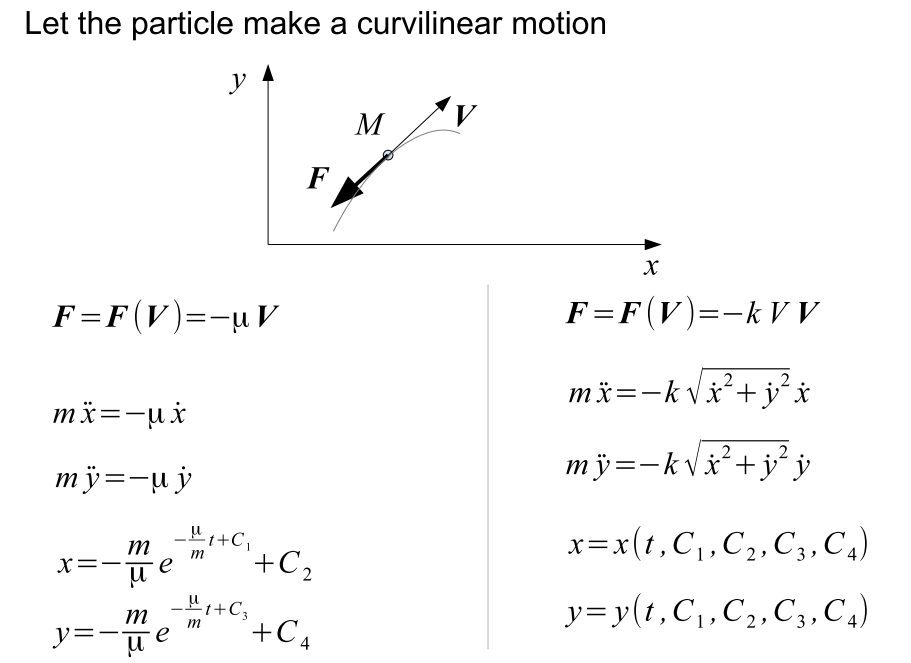
\includegraphics[height=5cm,width=1\textwidth,keepaspectratio]{image6.png}
            \label{fig:image6}
        \end{figure}
    \end{center}
\end{frame}

\begin{frame}[t]{Typical differential equations}
    \framesubtitle{Position dependent force}
    \vspace*{-0.6cm}
    \begin{center}
        \begin{figure}[H]
            \centering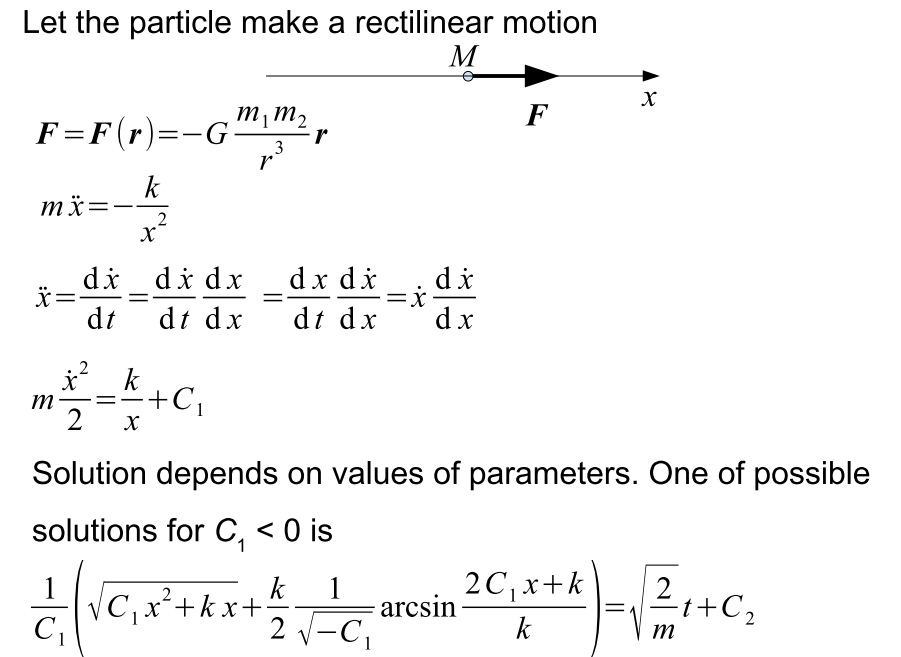
\includegraphics[height=5cm,width=1\textwidth,keepaspectratio]{image16.png}
            \label{fig:image16}
        \end{figure}
    \end{center}
\end{frame}

\begin{frame}[t]{Typical differential equations}
    \framesubtitle{Position and velocity dependent force}
    \vspace*{-0.6cm}
    \begin{center}
        \begin{figure}[H]
            \centering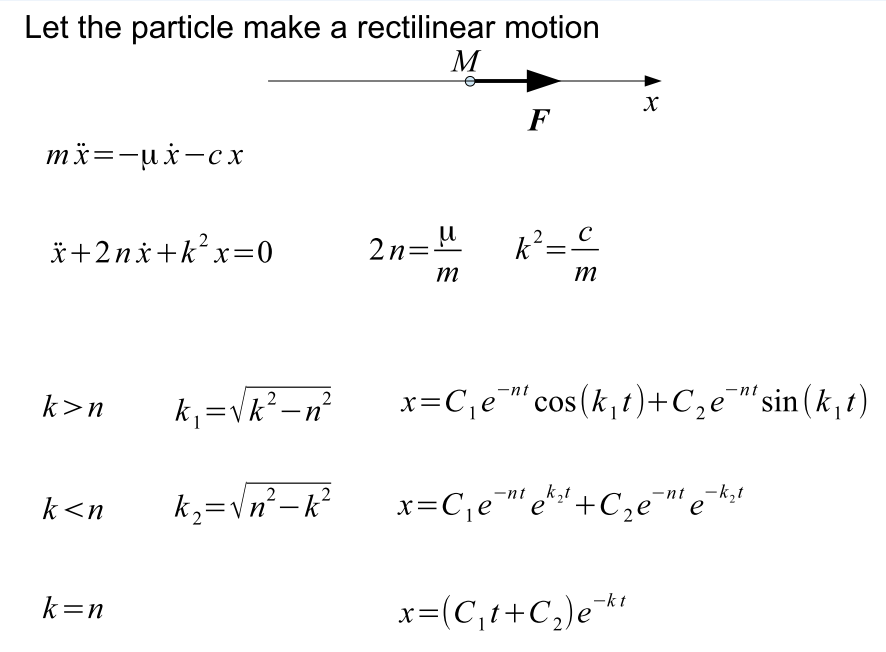
\includegraphics[height=5cm,width=1\textwidth,keepaspectratio]{image17.png}
            \label{fig:image17}
        \end{figure}
    \end{center}
\end{frame}


\section*{Tasks}

\begin{frame}[t]{2nd Newton Law for Inertial systmes}
\framesubtitle{}
\footnotesize
    \begin{tabular}{>{\centering\arraybackslash} m{1.5cm}|>{\centering\arraybackslash} m{3cm}|>{\centering\arraybackslash} m{3.5cm}|>{\centering\arraybackslash} m{2.2cm}|>{\centering\arraybackslash} m{1.7cm} } 
        \toprule
        \toprule
        \ExecuteMetaData[../../dynamics_methods_overview/dynamics_methods_overview]{top}
        \hline
        \ExecuteMetaData[../../dynamics_methods_overview/dynamics_methods_overview]{sndnewinert}
        \bottomrule
        \bottomrule
        \end{tabular}
\end{frame}

\begin{frame}[t]{Task 1 (mine)}
    \begin{minipage}{0.49\textwidth}
        The boat has an initial velocity $v_o$ and a mass $m$. Resistance force $F_c(v)$ also affects on the boat. You should:
        \begin{enumerate}
            \item Find an equation of motion of this boat.
            \item Find the time when the boat speed will be reduced twice.
        \end{enumerate}
    \end{minipage}
    \begin{minipage}{0.49\textwidth}
        \vspace{-0.8cm}
        \begin{figure}[H]
            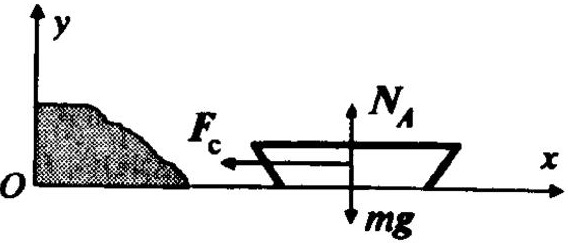
\includegraphics[height=5cm,width=1\textwidth,keepaspectratio]{lab9_task1_fig.jpg}\\
            \caption*{Task 1}
        \end{figure}
    \end{minipage}
\end{frame}

\begin{frame}[t]{Task 2 (yours)
    }
    \framesubtitle{}
        \begin{columns}[T,onlytextwidth]
            \begin{column}{0.49\textwidth}
                The body $D$ has a mass $m$. It moves up because of $F$ force. There is no friction between $D$ and ground.
                \medskip

                The task is to find an equation of $D$ motion.

                Needed variables: \\
                $m = 2,\ F_x = 12 \cos (3t)$;\\
                $\alpha = 30,\ v_0 = 4$.
                \bigskip

                \textit{Answer}: $x=4t-2.45t^2 - 0.67(\cos (3t)-1)$
            \end{column}
            \begin{column}{0.49\textwidth}
                \begin{figure}[H]
                    \centering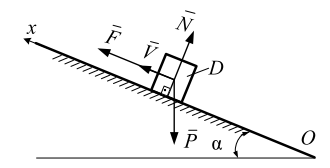
\includegraphics[height=5cm,width=1\textwidth,keepaspectratio]{image24.png}
                    \caption*{Task 2}
                    \label{fig:image24.png}
                \end{figure}
            \end{column}
        \end{columns}
\end{frame}

\begin{frame}[t]{2nd Newton Law for Non Inertial systmes}
    \framesubtitle{}
    \scriptsize
        \begin{tabular}{>{\centering\arraybackslash} m{1cm}|>{\centering\arraybackslash} m{1.8cm}|>{\centering\arraybackslash} m{3.5cm}|>{\centering\arraybackslash} m{2cm}|>{\centering\arraybackslash} m{4cm} } 
            \toprule
            \toprule
            \ExecuteMetaData[../../dynamics_methods_overview/dynamics_methods_overview]{top}
            \hline
            \ExecuteMetaData[../../dynamics_methods_overview/dynamics_methods_overview]{sndnewnoninert}
            \bottomrule
            \bottomrule
            \end{tabular}
    \end{frame}

\begin{frame}[t]{Task 3 (mine)}
    \begin{minipage}{0.69\textwidth}
        The figure shows a pipe $AB$, which rotates about a vertical axis $CD$ with a constant angular velocity $\omega$. The angle between $AB$ and $CD$ is always $45^\circ$.

        A small heavy ball is placed in the pipe. Determine the motion of the ball, assuming that its initial velocity is $0$ and the initial distance between the ball and a point $O$ equals $a$. Neglect friction. \bigskip

        \textit{Answer:} $OM=\dfrac{1}{2}(a-\dfrac{g\sqrt{2}}{\omega^2})(e^{0.5\omega t \sqrt{2}} + e^{-0.5\omega t \sqrt{2}}) + \dfrac{g\sqrt{2}}{\omega^2}$

    \end{minipage}
    \begin{minipage}{0.29\textwidth}
        % \vspace{-0.8cm}
        \begin{figure}[H]
            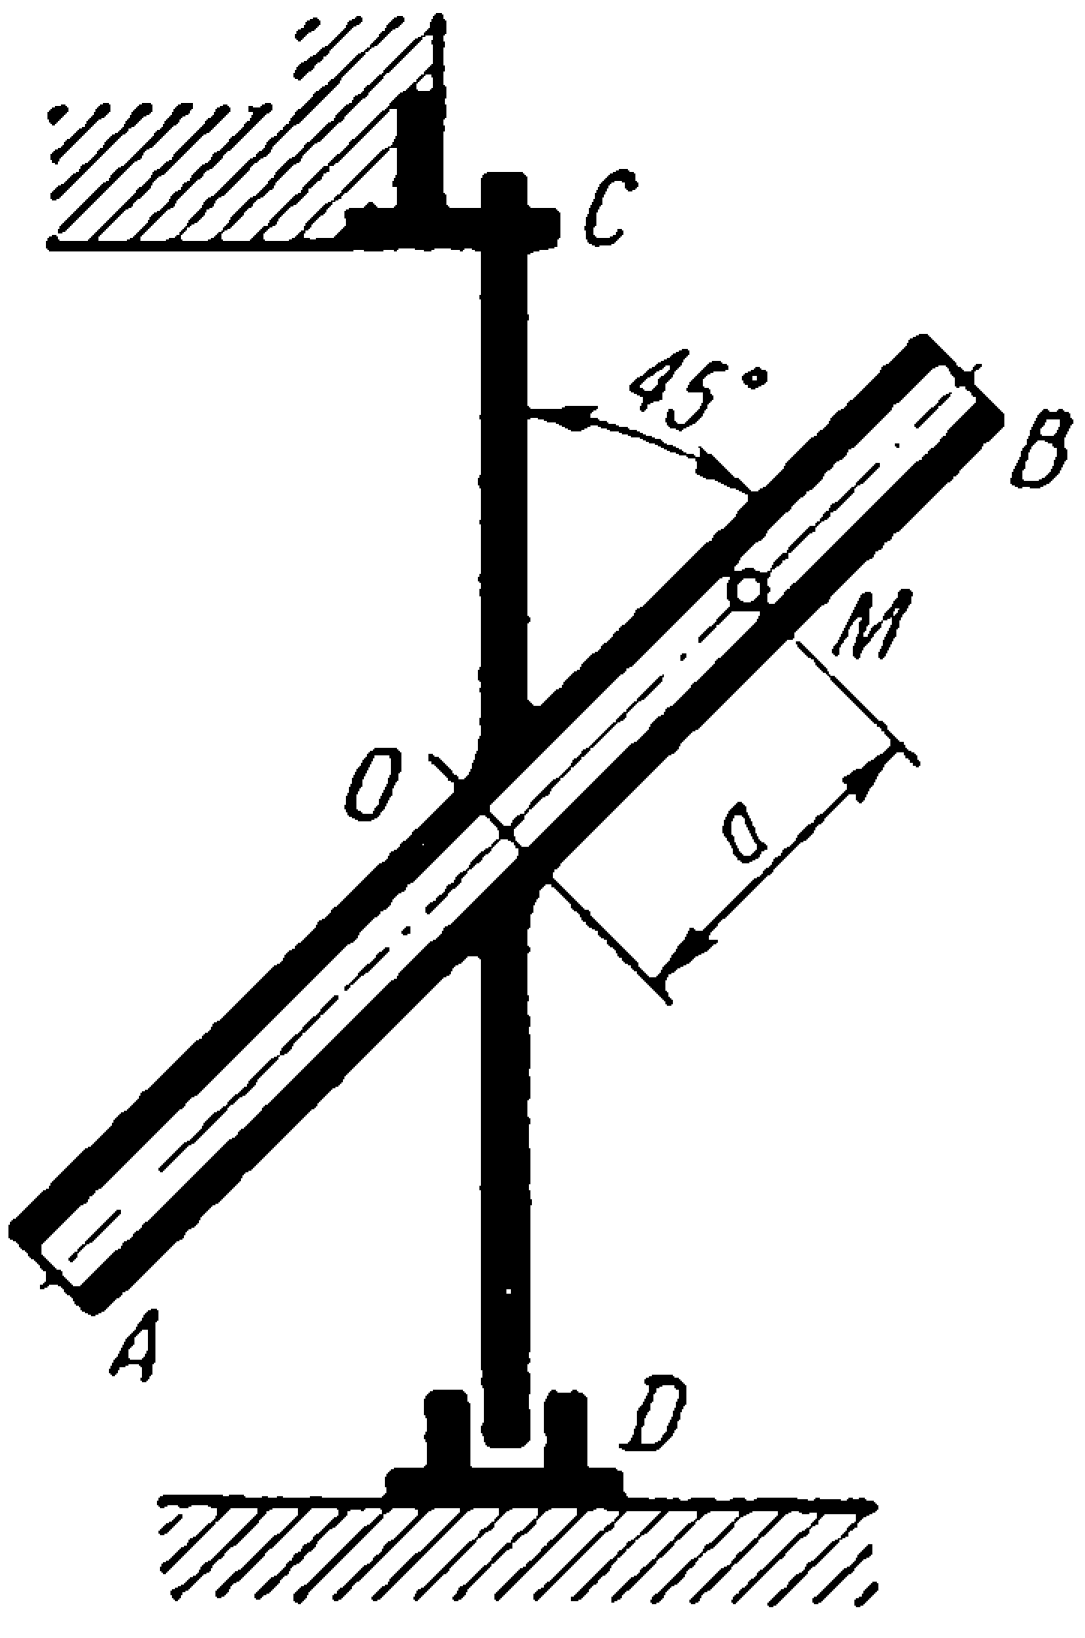
\includegraphics[height=5cm,width=1\textwidth,keepaspectratio]{lab9_task2_fig.png}\\
            \caption*{Task 3}
        \end{figure}
    \end{minipage}

\end{frame}

\begin{frame}[t]{Task 4 (yours): M (rus) 33.10}
    \framesubtitle{}
    \vspace*{-0.6cm}
    \begin{columns}[T,onlytextwidth]
        \begin{column}{0.49\textwidth}
            The horizontal tube $CD$ rotates with the constant angular velocity $\omega=const$ along $AB$ axis. There is a body $M$ inside the tube.

            The task is to find the velocity of $M$ related to the tube in a moment, when the body leaves the tube. No friction between $M$ and the tube.

            We know that the length of the tube is equal to $L$, the initial velocity is equal to zero $(v_0 = 0)$ and initial position was $x_0$.
            \bigskip

            \textit{Answer}: $v=\sqrt{L^2 - x_0 ^2 \omega}$
        \end{column}
        \begin{column}{0.49\textwidth}
            \begin{figure}[H]
                \centering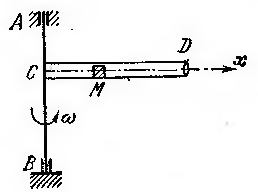
\includegraphics[height=5cm,width=1\textwidth,keepaspectratio]{image25.png}
                \caption*{Task 4}
                \label{fig:image25.png}
            \end{figure}
        \end{column}
    \end{columns}
\end{frame}

\fbckg{fibeamer/figs/last_page.png}
\frame[plain]{}
\end{document}